\documentclass[titlepage]{article}
\usepackage[pdftex]{graphicx}

% Title
\title{Lab 1: Simple Harmonic Motion}
\author{Milos Leposavic}

\begin{document}
\maketitle

\section{Objective of the Experiment}\label{sec:obj}
The purpose of this lab was to study the effects of Simple Harmonic Motion using springs and pendulums. We also got ourselves familiarized with the oscilloscope.

\section{Theory}\label{sec:theory}
When an object exhibits periodic motion, the object is said to be in \textbf{harmonic motion}. The fundamental type of this motion is known as Simple Harmonic Motion (SHM).\\
\\
A string that is stretched past its point of equilibrium and allowed to contract freely will exhibit Simple Harmonic Motion. Once observed, it's very easy to see a spring in such motion is periodic, and if we exclude all external forces, it would continue to move this way perpetually.\\
\\
A pendulum works the same way. Once pulled to one side and allowed to return to its equilibrium position, the pendulum will oscillate between it's point of equilibrium, showing a constant gain and loss of potential and kinetic energy. If we were to do this  in a vacuum, it would continue like this forever because there is no air resistance or any other forces that are stopping it.

\section{Equipment List}\label{sec:equipment_list}
\begin{itemize}
\item[*] Ring Stand
\item[*] Spring
\item[*] Masses
\item[*] Timer
\item[*] Function Generator
\item[*] DC Power Source
\item[*] Oscilloscope
\end{itemize}

\section{Procedure}\label{sec:procedure}
\subsection{Part A}\label{sub:part_a}
For the first part of the experiment we attached the spring to a ring stand and hung a mass from the end of the spring. We held the mass at the springs equilibrium point and then we let it drop so that the spring was allowed to oscillate. We recorder the time for 10 oscillations. We repeated this several times in order to obtain an average time. We did this same experiment five times with different masses.

\subsection{Part B}\label{sub:part_b}
For the second part we attached a string to the ring stand and hung a mass from the other end. We displaced the mass to one side so that the string was allowed to swing freely. Once again, we recorded the time for 10 oscillations. This was repeated several times to get an average time, and was repeated five times with different lengths of string.

\subsection{Part C}\label{sub:part_c}
In the last part of the lab we set the generator to a specific frequency of known value, and measurements were taken. This was done multiple times, and the measurements that we obtained were then used to compare the given frequency to the frequency read by the oscilloscope.

\section{Data}\label{sec:data}
\subsection{Part A}\label{sub:part_a}

Spring Oscillations
\begin{tabular}{cccccc}
\hline
Mass (g) & 10 & 20 & 30 & 40 & 50\\
\hline
Time (sec) & 3.60 & 4.58 & 5.62 & 6.15 & 7.04\\
\hline
$T$ & 0.360 & 0.458 & 0.562 & 0.615 & 0.704\\
\hline
$T^2$ & 0.129 & 0.209 & 0.315 & 0.378 & 0.495\\
\hline
\end{tabular}

\subsection{Part B}\label{sub:part_b}

Pendulum Oscillations
\begin{tabular}{cccccc}
\hline
Length (m) & .10 & .20 & .30 & .40 & .50\\
\hline
Time (s) & 6.81 & 9.33 & 11.05 & 11.98 & 13.98\\
\hline
$T$ & 0.681 & 0.933 & 1.105 & 1.198 & 1.398\\
\hline
$T^2$ & 0.463 & 0.870 & 1.220 & 1.435 & 1.954\\
\hline
\end{tabular}


\section{Analysis of Data}\label{sec:analysis_of_data}

\subsection{Part A}\label{sub:part_a}
The equation that we used to relate the mass and the spring to the time it takes to complete an oscillation is the equation for the period of oscillations and it is
\begin{equation}
	T = 2 \pi \sqrt{\frac{m}{k}}
\end{equation}
By squaring both sides of the equation, we get
\begin{equation}
	T^2 = \frac{4 \pi^2}{k} m
\end{equation}
When the time is squared, and the mass attached to the spring are plotted in a linear fashion, the slope of the line is equal to $\frac{4 \pi^2}{k}$. The value of $k$ can then be found by using the equation
\begin{equation}
	k = -\frac{mg}{x}
\end{equation}
\\
\\
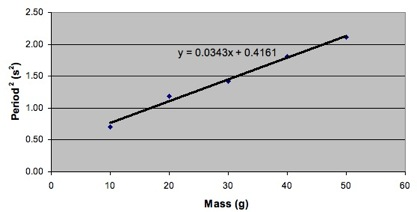
\includegraphics{graphA.jpg}
\\
Using the approximate slope we have calculated, we can derive the constant $k$.

\[
	0.0343 = \frac{4 \pi^2}{k}
\]
\[
	k = 1150.97
\]
The percent error can now be tabulated
\[
	\% Error = \frac{|1264.52 - 1150.97|}{1264.52} * 100 = 8.98\%
\]

\subsection{Part B}\label{sub:part_b}
We can relat the three main factors of this experiment, the gravitational acceleration, the period of the oscillation and the length of the string of the pendulum with thsis equation
\begin{equation}
	T = 2 \pi \frac{L}{g}
\end{equation}
With a little manipulation to the equation we can get a more useful one
\begin{equation}
	T^2 = \frac{4 \pi^2}{g} L
\end{equation}
Once this function is plotted, it yields a linear regression, with the slope of the line being represented by $\frac{4 \pi^2}{g}$.
\\
\\
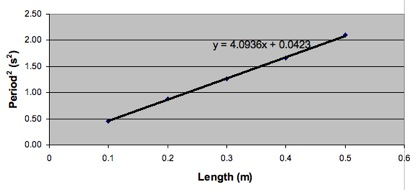
\includegraphics{graphB.jpg}
\\
Now that we have an approximate regression line, we can use this to determine the value of $g$

\[
	4.0936 = \frac{4 \pi^2}{g}
\]
\[
	g = 9.644 \frac{m}{s^2}
\]

Now, once we have $g$ we determine the percent error
\[
	\% Error = \frac{|9.81 - 9.64|}{9.81} * 100 = 1.69\%
\]

\subsection{Part C}\label{sub:part_c}

In order to get the oscilloscope working properly, it was necessary for us to first, zero out the oscilloscope. By zeroing out a scale or any other measuring device, we are allowed to read accurate results.\\
\\
Next, we set the DC power supply to 5 volts and the oscilloscope showed us a flat line. This makes sense, because the amount of voltage was had a constant value over time. Which means that if we increased and decreased the value of the voltage, the line would translate itself up or down, respectively. By altering the VOLT/DIV knob, the location of the line changed as well. This changes the scale of the grid lines.\\
\\
By changing the oscilloscope channel, we were able to view the AC waveform, rather than the DC waveform. By altering the SEC/DIV knob, we changed the time scale so that only a few cycles of the waveform could be seen. We measured the time it took the wave to make one complete cycle, and by taking the inverse, we are left with the frequency. The result we obtained was 1429 Hz. After this, we changed the vertical position of the wave so that it would line up with the grid lines. Amplitude was determined by counting the grid lines from the peak of the wave to 0.\\
\\
The function generator was set to 1500 Hz, and we calculated the value of 1429 Hz. Based on these results we calculated the percent error
\[
	\% Error = \frac{|1500 - 1429|}{1500} * 100 = 4.7\%
\]

\section{Discussion of Results}\label{sec:discussion_of_results}
\subsection{Part A}\label{sub:part_a}
We the calculation done and with the data obtained we calculated the spring constant. It came to be $k = 1264.52$. The \% Error of $8.98\%$ is pretty decent. I think that the error is kind of big because we were timing the oscillations by eye, rather than using something more accurate, like a photo gate. Because of this, it's understandable to have a slight discrepancy between the true value.

\subsection{Part B}\label{sub:part_b}
In the second part we calculated the value of $g$ to be $9.64 \frac{m}{s^2}$. Our \% Error of $1.69\%$ is very small in my opinion, because there are a lot of focres outside the system that could alter our obtained data. Just like for the above obtained data, I think the largest amount of the error is coming from the fact that we judged the oscillations by eye, and had to manually determine the time, rather than using photo gates.

\subsection{Part C}\label{sub:part_c}
For the last parttThe measured amplitudes for both the DC and AC sources were very accurate and consistent. The calculated frequency for the wave was 1429 Hz, despite the fact that the function generator was set to 1500 Hz. The error is 4.7\%. I think that this error was most likely our fault because we could not read the exact measurement off the oscilloscope.

\section{Conclusions}\label{sec:conclusions}
The relatively accurate and consistent results provided by our data reinforces the validity of the equations presented to us in class. You can see this by looking at the tables for Part A and B. It is very clear that the linear regression is quite accurate based on our data, and the linear regression calculates the constants $k$ and $g$ accurately. The cause for error is obviously on our part, considering we could've used for more accurate methods of timing than the human eye and hand.

\end{document}

